\section{Results} \label{sec:results}

\begin{figure}[h]%[thpb]
\centering
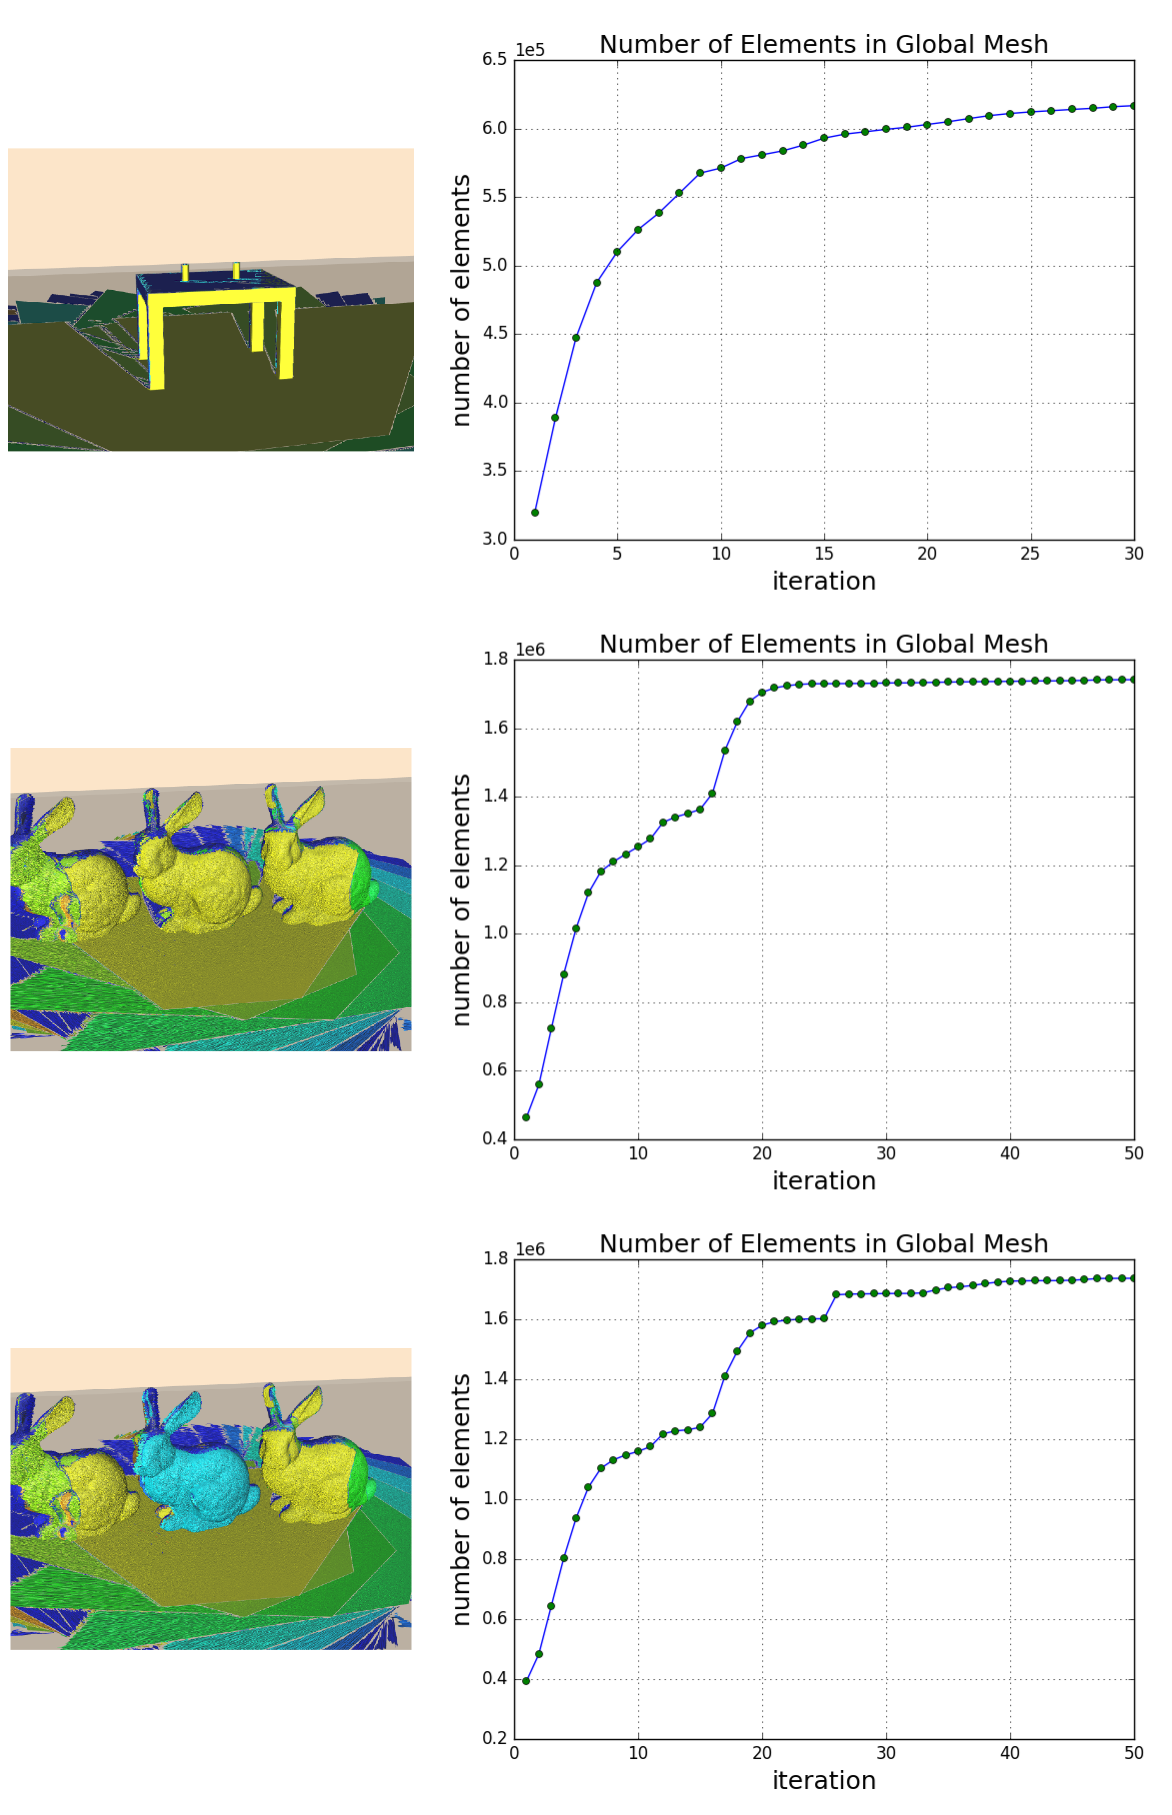
\includegraphics[width=0.48\textwidth]{figures/diagram_run123_gm.png}
\caption{Global mesh results.}
\label{fig:run1d}
\end{figure}

Results of all experimental runs. For each run: Top-left is the global mesh,
top-middle is the novel surface, top-right is the number of elements in the
global mesh, bottom-left what we actually saw, bottom-middle what we expected to
see, bottom-left threshold of the difference between expected and actual.
